\section{局域网：先找到机器人，再记住它的名字}
\label{sec:deploy-lan}

远程连接首先得回答一个朴素的问题：机器人在哪里？这里问的是网络地址。把笔记本和机载电脑接到队内路由器后，路由器通常用动态主机配置协议（Dynamic Host Configuration Protocol，DHCP）为它们分配地址。例如，笔记本是 \texttt{192.168.50.10/24}，机器人是 \texttt{192.168.50.20/24}；\texttt{/24} 对应子网掩码 \texttt{255.255.255.0}，这个例子里二者属于同一子网。\textbf{这些只是示例地址，动手时以实际输出为准}，不要把书上的地址直接写进已有网络。

在机载电脑本地终端运行 \texttt{ip -br address}，查看处于 \texttt{UP} 状态的网口及其地址；\texttt{lo} 上的 \texttt{127.0.0.1} 只指向本机，不能拿给笔记本连接。\texttt{ip route} 查看路由，含 \texttt{default via} 的一行表示默认出口。只在同一子网内调试不要求有互联网，但两台设备必须能够互相通信：校园网、访客 Wi-Fi 或路由器的客户端隔离，可能让“连着同一个 Wi-Fi”仍然无法互访。

\begin{example}[按地址检查局域网连通性]
先在机器人本地查看：
\begin{tbash}
ip -br address
ip route
\end{tbash}
假设确认有线地址是 \texttt{192.168.50.20/24}，再到笔记本的 Linux 终端运行：
\begin{tbash}
ip -br address
ip route get 192.168.50.20
ping -c 3 192.168.50.20
ssh rm@192.168.50.20
\end{tbash}
这里 \texttt{rm} 是机器人上的登录用户名；SSH 服务的安装与登录见第~\ref{sec:deploy-ssh}~节。\texttt{ip route get} 应显示通往机器人的实际网卡与源地址；\texttt{ping} 收到回复说明此刻 ICMP 能往返，但不能证明 SSH 已启动。反过来，防火墙也可能禁 ICMP 而允许 SSH，因此 \texttt{ping} 不通时还要结合实际服务判断。
\end{example}

如果 IP 能连，每次还得问“今天机器人分到几号地址”就有点麻烦了。我们可以给机器人取一个稳定的\textbf{主机名（Hostname）}，例如 \texttt{rm-robot}。但名字不会自动变成地址：直接写 \texttt{ssh rm@rm-robot}，需要本地 DNS、搜索域或 \path{/etc/hosts} 等机制能够解析这个名字。

在常见的小型局域网内，更方便的是多播 DNS（Multicast DNS，mDNS）：用 \texttt{rm-robot.local} 在本地链路查询机器人的地址。Linux 常用 \href{https://avahi.org/}{Avahi} 发布名字，并通过系统解析器或 \href{https://github.com/avahi/nss-mdns}{nss-mdns} 让普通程序也能解析 \texttt{.local}。它要求目标端发布名字、客户端支持解析，且网络放行本地 mDNS 多播；通常不能指望它跨 VLAN、跨路由或穿过隔离网络。

\begin{example}[让 Ubuntu 22.04 机器人能按名字访问]
前提是两端已接入可互访的局域网，机器人已具有不同于队内其他设备的名字。在\textbf{机器人本地终端}配置：
\begin{tbash}
sudo hostnamectl set-hostname rm-robot
sudo apt update
sudo apt install avahi-daemon libnss-mdns
sudo systemctl enable --now avahi-daemon
hostnamectl --static
\end{tbash}
若 \path{/etc/hosts} 的 \texttt{127.0.1.1} 行仍写着旧主机名，用 \texttt{sudoedit /etc/hosts} 同步改为新名，保留原有其他条目。修改名字会影响后续连接，请在本地完成后再重新建立远程会话。

在\textbf{Ubuntu 笔记本}安装同样两个包并启动 Avahi，然后测试：
\begin{tbash}
getent hosts rm-robot.local
ssh rm@rm-robot.local
\end{tbash}
\texttt{getent hosts} 走系统的名字解析路径，出现机器人的地址后才继续 SSH。Windows 或 macOS 笔记本也可以先试 \texttt{ssh rm@rm-robot.local}；能否解析取决于该系统及网络配置，失败时先用已核实的 IP 连接。
\end{example}

如果数字 IP 可用但 \texttt{.local} 不可用，故障就在名字解析这一步附近。先看 \texttt{systemctl status avahi-daemon}，再看 \path{/etc/nsswitch.conf} 的 \texttt{hosts:} 行是否包含可用的 mDNS 解析模块；Ubuntu 常见的是 \texttt{mdns4\_minimal}。不要直接拿网上的一整行覆盖本机配置，因为还可能存在 \texttt{resolve}、\texttt{myhostname} 等系统模块。\texttt{nslookup} 直接询问 DNS 服务器，不能用它的失败单独判定 mDNS 失败；这也是这里选 \texttt{getent} 的原因。

\begin{exercise}\label{ex:deploy-lan}
在自己的网络记录两端地址、前缀及通往机器人的出口网卡，分别用数字 IP 与 \texttt{.local} 名字尝试 SSH。若只有名字失败，给出两项针对名字解析的检查；若都失败，给出两项针对链路、子网或隔离的检查。没有机器人时可用第二台练习电脑，注明替代条件。
\end{exercise}

\section{一根网线直连：不用路由器也能调车}
\label{sec:deploy-wired}

训练场没有可靠的 Wi-Fi，或者临近比赛不便使用无线网络时，先别急着搬出显示器。\textbf{只要机器人系统、网卡和 SSH 还正常，一根网线直连也能使用同样的远程工具}。笔记本没有网口，就加一个 USB 以太网适配器；它提供网卡，不会自动给机器人分配地址。普通笔记本与机器人直连时通常没有 DHCP 服务器，所以我们给两端各设一个固定地址。

下面只演示\textbf{两端都由 NetworkManager 管理的以太网接口}。Ubuntu Desktop 常见这种配置；有些机载 Ubuntu Server 使用 systemd-networkd/Netplan，此时 \texttt{nmcli device status} 可能显示接口未托管，应按现有网络管理方式配置，不能一边保留原管理器一边强行接管。\href{https://networkmanager.pages.freedesktop.org/NetworkManager/NetworkManager/nm-settings-nmcli.html}{NetworkManager 配置参考}列出了地址、默认路由和连接配置的含义。

\begin{note}
切换网卡配置会断开该网卡原来的连接。先在两端本地终端或硬件 KVM 中操作，记录当前连接名，并确认示例子网 \texttt{192.168.77.0/24} 不与现有 LAN、VPN 路由重叠。不要通过唯一的 SSH 会话修改它赖以连接的网卡；也不要在机器人运动时挂着调试线。
\end{note}

\begin{example}[新建独立的直连配置，保留原配置]
先在\textbf{两端}运行以下只读命令，记下以太网接口名和当前连接名：
\begin{tbash}
nmcli device status
nmcli connection show --active
ip route
\end{tbash}
下面假设笔记本网口是 \texttt{enp3s0}，机器人网口是 \texttt{enp2s0}；必须替换为各自实际名称。先插好两端网线，避免启用以太网配置时因没有链路而失败，再在\textbf{笔记本}创建配置并启用：
\begin{tbash}
sudo nmcli connection add type ethernet ifname enp3s0 \
  con-name rm-direct connection.autoconnect no \
  ipv4.method manual ipv4.addresses 192.168.77.1/24 \
  ipv4.never-default yes ipv6.method disabled
sudo nmcli connection up rm-direct
\end{tbash}
\Needspace{9\baselineskip}
再在\textbf{机器人}本地创建它的配置并启用：
\begin{tbash}
sudo nmcli connection add type ethernet ifname enp2s0 \
  con-name rm-direct connection.autoconnect no \
  ipv4.method manual ipv4.addresses 192.168.77.2/24 \
  ipv4.never-default yes ipv6.method disabled
sudo nmcli connection up rm-direct
\end{tbash}
这两段均\textbf{没有设置网关和 DNS}；\texttt{never-default yes} 使这个配置不抢默认路由，笔记本仍可用自己的其他网络上网。\texttt{autoconnect no} 表示下次需手动启用该练习配置；这里暂时禁用该配置的 IPv6，只为让初学实验集中观察 IPv4，并不要求全系统禁用 IPv6。

双方配置启用后，在笔记本验证：
\begin{tbash}
ip route get 192.168.77.2
ping -c 3 192.168.77.2
ssh rm@192.168.77.2
\end{tbash}
结果应显示直连网卡，SSH 应登录机器人；两端没有接入互联网也能完成这些操作。结束时，在两端本地分别执行：
\begin{tbash}
sudo nmcli connection down rm-direct
sudo nmcli connection up "原来的连接名"
\end{tbash}
最后一行的名字换成实验前记录的值；若接口原先没有连接，就无需恢复一个不存在的配置。确认不再需要练习配置后，可用 \texttt{sudo nmcli connection delete rm-direct} 删除\textbf{本次新建的配置}，不要删除原配置。
\end{example}

Windows 笔记本可以在“网络连接”中找到对应的以太网适配器，打开 IPv4 属性，将地址设为 \texttt{192.168.77.1}、掩码设为 \texttt{255.255.255.0}，网关与 DNS 留空；机器人侧仍按上述配置。练习前记录原设置，结束后恢复原来的自动获取或固定配置。注意选择真正插着网线的适配器，别把 Wi-Fi 或 Tailscale 的虚拟网卡改了；具体界面可查\href{https://support.microsoft.com/en-us/windows/experience/connectivity-networking/essential-network-settings-and-tasks-in-windows}{微软的 TCP/IP 设置说明}。

\begin{exercise}\label{ex:deploy-wired}
写一张双端直连配置卡：列出实际接口名、原连接名、两端地址/前缀及恢复命令。在停机的练习设备完成直连，记录路由与 SSH 结果，并说明为什么无需填写网关。如果没有可用网口，只提交配置卡并明确“未实接”，不能用纸面方案替代接线验收。
\end{exercise}

\section{不在同一局域网：用 Tailscale 建立远程维护通道}
\label{sec:deploy-tailscale}

机器人在实验室，你在宿舍；两边都有互联网，却接着不同路由器。这时机器人的 \texttt{192.168.*.*} 私有地址不能直接从外部访问，\texttt{.local} 也通常到不了。\textbf{Tailscale} 可以在获准加入的设备之间建立加密网络，设备组成的网络称为 Tailnet。你仍然运行原来的 SSH 或远程桌面，只是把目标换成 Tailscale 地址或名字，不必把 SSH 端口直接转发到公网。

图~\ref{fig:deploy-network-paths}~把三种情况放在一起：局域网使用现有 LAN 地址；网线直连使用约好的静态地址；跨网络时则在双方联网基础上增加 Tailscale。它们解决“怎么到达目标”，SSH 和远程桌面解决“到达后怎样操作”。

\begin{figure}[htbp]
  \centering
  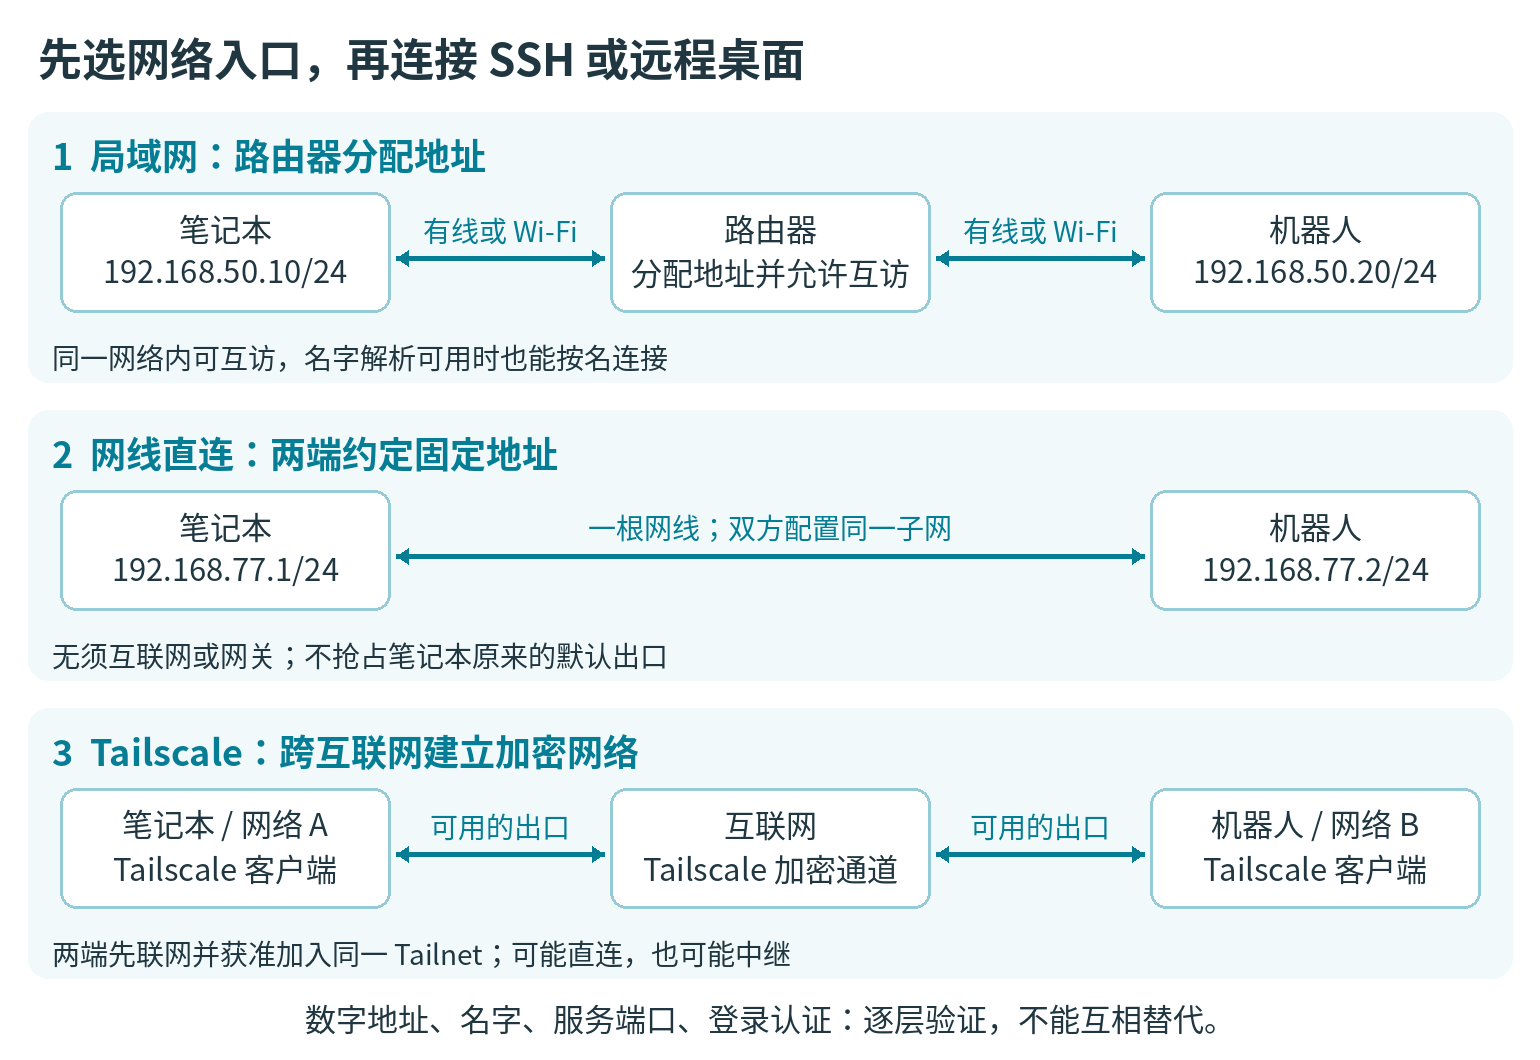
\includegraphics[width=0.94\textwidth]{deployment/network_paths_revised.png}
  \caption{三种网络入口，最终都连接到机器人上已运行的服务。地址为教学示例；跨网络的 Tailscale 连接可能直达，也可能经过中继。}
  \label{fig:deploy-network-paths}
\end{figure}

\subsubsection{安装、加入同一个 Tailnet，再验证地址}
先和队内负责人确认使用哪个 Tailnet、怎样给成员授权。个人练习可在两端登录同一账户；团队设备应按管理员的成员、标签及访问策略管理，不能把共享登录密码写进教材工程。\href{https://tailscale.com/download}{官方下载页}提供 Windows、macOS 和 Linux 客户端；Windows/macOS 笔记本安装后从托盘或菜单栏登录。

\begin{example}[在 Ubuntu 22.04 机器人安装 Tailscale]
本例采用\href{https://pkgs.tailscale.com/stable/#ubuntu-2204}{官方 Ubuntu 22.04 稳定仓库}，而不是固定某个过时安装包。先在机器人本地或已有 SSH 中确认系统版本：
\begin{tbash}
. /etc/os-release
printf '%s %s\n' "$ID" "$VERSION_CODENAME"
\end{tbash}
下面命令\textbf{只用于输出为 \texttt{ubuntu jammy} 的环境}；其他版本按官方页面选择对应仓库。添加仓库需要管理员权限，会改变系统的软件源：
\begin{tbash}
sudo apt update
sudo apt install curl ca-certificates
curl -fsSL https://pkgs.tailscale.com/stable/ubuntu/jammy.noarmor.gpg \
  -o /tmp/tailscale-jammy-key.gpg
curl -fsSL https://pkgs.tailscale.com/stable/ubuntu/jammy.tailscale-keyring.list \
  -o /tmp/tailscale-jammy.list
\end{tbash}
确认下载成功，查看 \texttt{cat /tmp/tailscale-jammy.list}，其中应指向官方稳定源、\texttt{jammy} 与签名密钥路径；若已配置 Tailscale 软件源，先核对现有设置，不要重复添加。再安装密钥和源文件：
\begin{tbash}
sudo install -d -m 0755 /usr/share/keyrings
sudo install -m 0644 /tmp/tailscale-jammy-key.gpg \
  /usr/share/keyrings/tailscale-archive-keyring.gpg
sudo install -m 0644 /tmp/tailscale-jammy.list \
  /etc/apt/sources.list.d/tailscale.list
sudo apt update
sudo apt install tailscale
sudo systemctl enable --now tailscaled
sudo tailscale up
\end{tbash}
终端会给出登录链接。机载电脑没开浏览器也没关系，在自己的笔记本打开该链接，用计划加入的账户登录，并按管理员要求完成设备批准。笔记本若也是 Ubuntu，同样按其系统版本安装并登录。

在\textbf{机器人}运行：
\begin{tbash}
tailscale status
tailscale ip -4
\end{tbash}
确认设备已登录，记下它实际获得的 Tailscale IPv4 地址。在\textbf{笔记本}运行下面命令；\texttt{100.88.0.20} 仅为示例，必须换成刚才的实际地址：
\begin{tbash}
tailscale status
tailscale ping 100.88.0.20
ssh rm@100.88.0.20
\end{tbash}
\texttt{status} 列出网络中的可见设备和状态；\texttt{tailscale ping} 检查两端 Tailscale 进程的通信路径，可能显示直连，也可能显示中继。它成功仍不等于 SSH 的端口、账户和权限都正常，最后必须用真正的 SSH 登录验证。
\end{example}

\subsubsection{MagicDNS：跨网络也可以用名字}
Tailscale 的 \textbf{MagicDNS} 为设备维护名字。管理员在管理控制台的 DNS 页面确认 MagicDNS 已启用，如图~\ref{fig:deploy-magicdns}；再从设备页面读取机器人的实际设备名及完整域名。它们可能与 Linux 主机名不同，重名时尤其要核对，不能靠猜。

\begin{figure}[htbp]
  \centering
  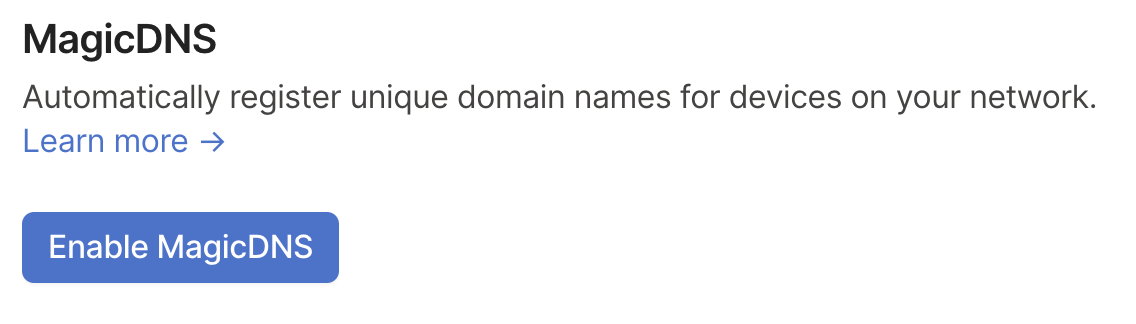
\includegraphics[width=0.84\textwidth]{deployment/tailscale_magicdns.png}
  \caption{Tailscale 官方文档中的 MagicDNS 启用入口。先看开关状态，再查设备名；已启用的网络无需重复操作。图片来源：\href{https://tailscale.com/docs/features/magicdns}{Tailscale MagicDNS 文档}，界面随版本可能调整。}
  \label{fig:deploy-magicdns}
\end{figure}

\begin{example}[区分两套名字，并检查解析]
假设 Tailscale 控制台显示机器人名为 \texttt{rm-robot}，且客户端接受 Tailnet DNS 配置，可在笔记本运行：
\begin{tbash}
tailscale ping rm-robot
ssh rm@rm-robot
\end{tbash}
若短名与局域网名字冲突，改用控制台显示的完整 MagicDNS 域名。例如 \path{rm-robot.tail-demo.ts.net}，其中 \path{tail-demo} 要换成自己的域名部分，再用实际 Tailscale 数字地址作对照。\path{rm-robot.local} 属于前面的本地 mDNS，后缀为 \path{ts.net} 的完整设备名属于 MagicDNS，二者的解析范围与前提不同。
\end{example}

\subsubsection{连通、授权与赛前检查要分别确认}
本章沿用的是\href{https://tailscale.com/docs/reference/ssh-over-tailscale}{通过 Tailscale 网络访问普通 OpenSSH}：机载电脑上的 \texttt{sshd} 继续负责 SSH 登录认证。另一项名为\href{https://tailscale.com/docs/features/tailscale-ssh}{Tailscale SSH}的功能会接管 Tailnet 上的 SSH 身份与授权，需要专门启用与配置。本章不执行 \texttt{tailscale set --ssh}，免得你在还没理清认证时把两条路线混在一起。

访问还会受到 Tailnet 的 Grants/ACL、设备批准及目标主机防火墙约束。若 \texttt{tailscale ping} 成功而 SSH 超时，核对目标 22 端口、\texttt{sshd}、主机防火墙和 Tailnet 的访问规则；若报 \texttt{Permission denied}，先回到 SSH 账户与密钥。\href{https://tailscale.com/docs/reference/troubleshooting/network-configuration/tcp-connection-two-devices}{官方连通性排错文档}说明了 Tailscale 自身通信与主机 TCP 服务之间的区别。

部署机器人时，还要在控制台检查\href{https://tailscale.com/docs/features/access-control/key-expiry}{设备密钥到期时间}。到期会中断设备连接，重新认证可能使当前远程会话掉线；提前在有本地或有线备用入口时处理。管理员可以对受信任的长期设备关闭密钥到期，但同时需要安排设备丢失后的撤销，不应把关闭到期当成所有设备的必选项。

\begin{conclusion}
局域网名字需要可用的本地解析；\texttt{.local} 通常只在本地链路生效；MagicDNS 依赖 Tailnet 及其 DNS 配置。先用数字地址定位网络问题，再查名字，最后查服务与认证。

Tailscale 适合跨网络维护，不会凭空创造互联网。双方断网、出口封锁或中继链路不可用时，不能保证远程连接；比赛前应实测并准备有线入口。SSH 能连接也不能推出 ROS 2 的自动发现、多播通信或大带宽相机流已可用；这些需要按卷二的通信机制另行配置与验收。
\end{conclusion}

\begin{exercise}\label{ex:deploy-tailscale}
在获准的 Tailnet 内记录机器人实际 Tailscale 地址、设备名、MagicDNS 完整域名与密钥到期状态。把笔记本切到另一条互联网连接，依次验证 \texttt{status}、\texttt{tailscale ping} 和 SSH；说明各自成功能证明什么。没有获准账户或第二条网络时，列出待办与缺少的条件，不能宣称跨网测试已通过。
\end{exercise}
